
\subsection{Meshes}

Describe meshes and material properties used for testing.

\begin{figure}
	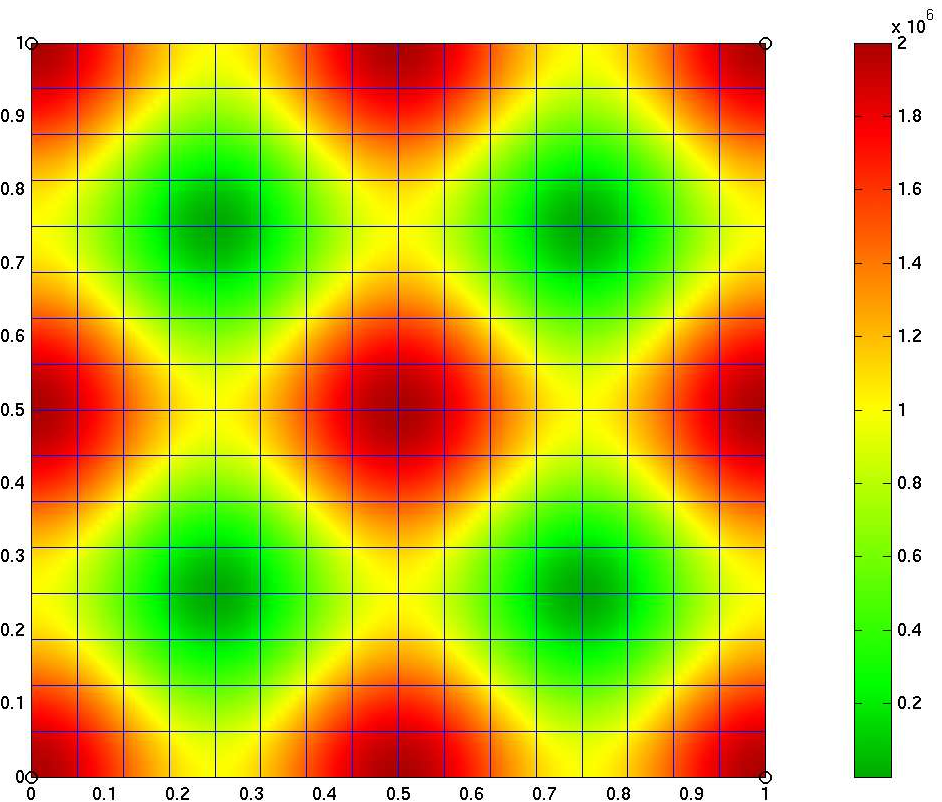
\includegraphics[width=0.45\textwidth]{figs/box}
	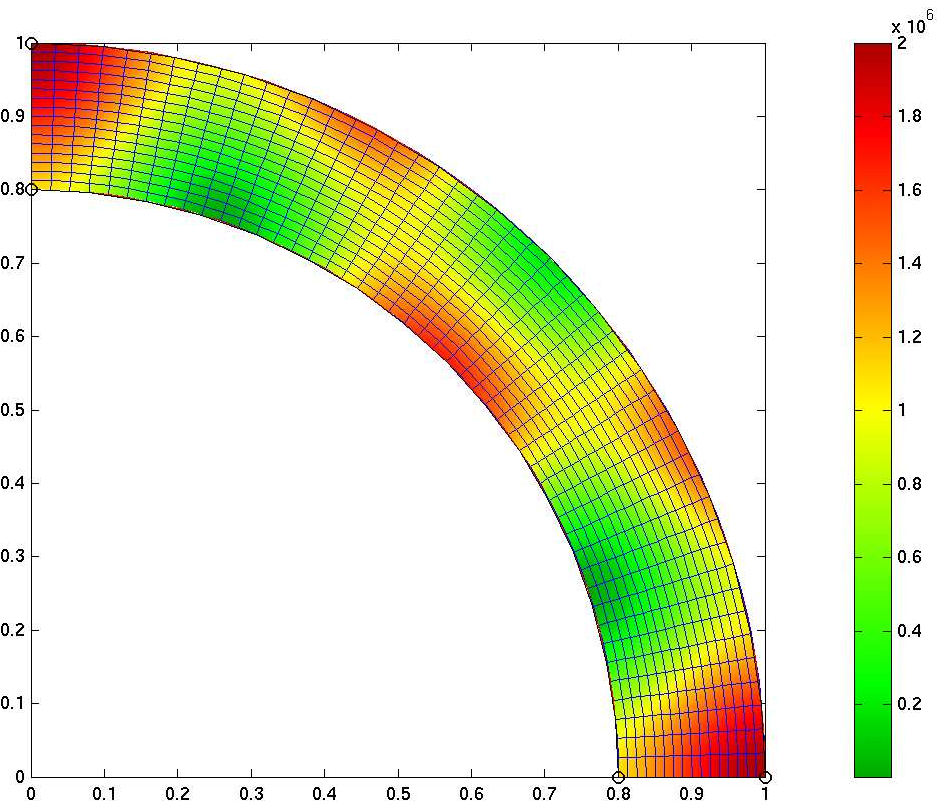
\includegraphics[width=0.45\textwidth]{figs/fan}
	\caption{\label{fig:mesh2d} The 2D meshes used for the tests.}
\end{figure}

\begin{figure}
	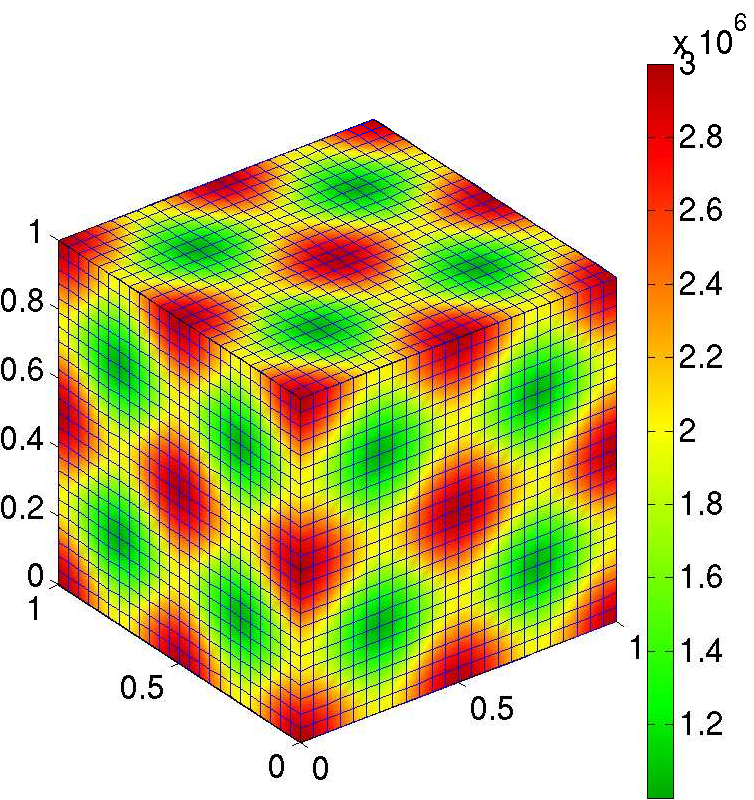
\includegraphics[width=0.45\textwidth]{figs/box3a}
	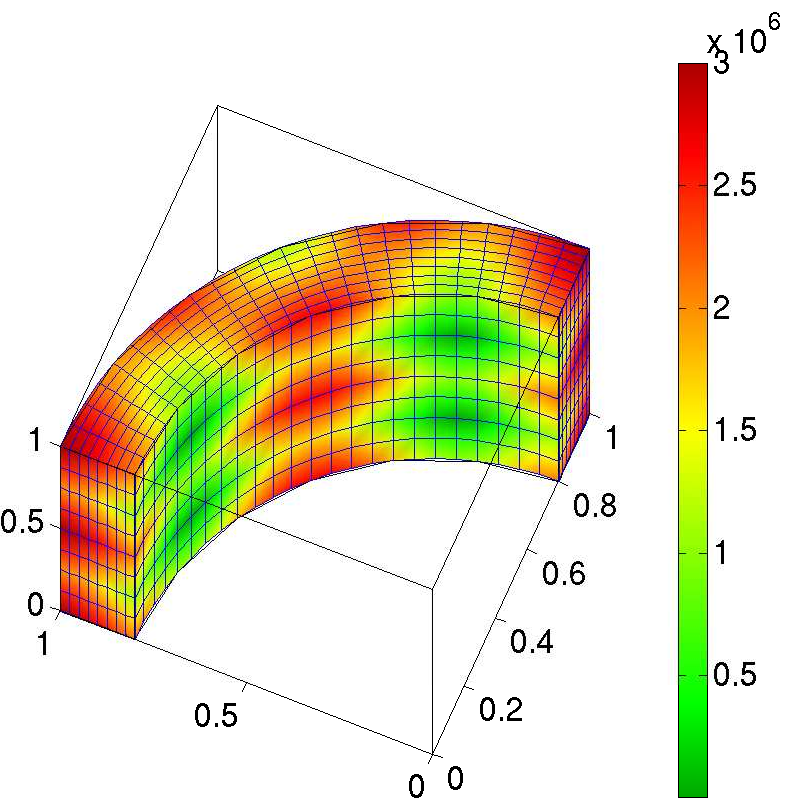
\includegraphics[width=0.45\textwidth]{figs/fan3a}
	\caption{\label{fig:mesh3d} The 3D meshes used for the tests.}
\end{figure}


\begin{table}
  \caption{\label{tab:homg} Number of CG iterations/v-cycles to converge to a relative tolerance of $10^{-8}$ for $h$-Multigrid applied to high-order operators on a rectangular domain. A total of 3 grids were used, the finest grid was $32\times 32$, and the coarsest was $8\times 8$.}
		\centering
    \begin{tabular}{|l|c|c|c|c|c|c|} 
	    \hline
				    & \multicolumn{3}{c|}{Multigrid} & \multicolumn{3}{c|}{MG pCG}\\  \cline{2-7}
			order & \scriptsize Jacobi(3)  &\scriptsize  Chebyshev(3)  &\scriptsize SSOR(2) &\scriptsize Jacobi(3)  &\scriptsize  Chebyshev(3)  &\scriptsize SSOR(2) \\
			\hline
				1 & 6 &  5 & 4  &  4  & 4  & 4 \\ 
	    	2 & 7 &  9 & 4  &  5  & 6  & 4 \\
				3 & 8 & 22 & 5  &  6  & 10 & 4 \\
				4 & - & 48 & 8  & 43  & 15 & 6 \\
				5 & - & 150 & 12 & 295 & 27 & 8 \\
				6 & - & - & 27  & - & 51 & 12 \\
				7 & - & - & 81 & - & 105 & 21 \\
				8 & - & - & 298 & - & 204 & 39 \\
			\hline
	  \end{tabular}
\end{table}

\begin{table}
  \caption{\label{tab:hpmg} Number of CG iterations/v-cycles to converge to a relative tolerance of $10^{-8}$ for $hp$-Multigrid applied to high-order operators on a rectangular domain. Starting with a $32\times 32$ high-order grid, we first coarsen in $p$ till $p=1$, and then coarsen in $h$. The coarsest grid in all cases is a $8\times 8$ grid with $p=1$}
		\centering
		\begin{tabular}{|l|c|c|c|c|c|c|} 
	    \hline
				    & \multicolumn{3}{c|}{Multigrid} & \multicolumn{3}{c|}{MG pCG}\\  \cline{2-7}
			order & \scriptsize Jacobi(3)  &\scriptsize  Chebyshev(3)  &\scriptsize SSOR(2) &\scriptsize Jacobi(3)  &\scriptsize  Chebyshev(3)  &\scriptsize SSOR(2) \\
			\hline
				1 & 6  &  5 &  4 & 4 & 4 & 4 \\ 
	    	2 & 7 & 9  & 4 & 5 & 6 & 4 \\
				%3 & 8 & 24 & 5 & 6 & 11 & 4 \\
				4 & - & 46 & 7 & 39 & 15 & 5 \\
				%5 & - & 178 & 13 & - & 28 & 8 \\
				%6 & - & - & 24 & - & 51 & 12 \\
				%7 & - & - & 70 & - & 105 & 19 \\
				8 & - & - & 267 & - & 182 & 36 \\
			\hline
	  \end{tabular}
\end{table}


\begin{table}
  \caption{\label{tab:homg} Number of CG iterations/v-cycles to converge to a relative tolerance of $10^{-8}$ for $h$-Multigrid applied to high-order operators on a fan domain. A total of 3 grids were used, the finest grid was $48\times 16$, and the coarsest was $12\times 4$.}
		\centering
    \begin{tabular}{|l|c|c|c|c|c|c|} 
	    \hline
				    & \multicolumn{3}{c|}{Multigrid} & \multicolumn{3}{c|}{MG pCG}\\  \cline{2-7}
			order & \scriptsize Jacobi(3)  &\scriptsize  Chebyshev(3)  &\scriptsize SSOR(2) &\scriptsize Jacobi(3)  &\scriptsize  Chebyshev(3)  &\scriptsize SSOR(2) \\
			\hline
      1 & 7  & 8  & 4 & 5 & 6 & 4 \\ 
	    2 & 9  & 12 & 5 & 6 & 7 & 4 \\	
			3 & 10 & 26 & 5 & 7 & 12 & 4 \\
      4 & -  & 54 & 8 & 136 & 17 & 6 \\
      5 & - & 171 & 14 & - & 31 & 8 \\
      6 & - & - & 42 & - & 53 & 15 \\
      7 & - & - & 146 & - & 109 & 29 \\
      8 & - & - & -  & - & -  & 85 \\
      \hline
	  \end{tabular}
\end{table}


\begin{table}
  \caption{\label{tab:hpmg} Number of CG iterations/v-cycles to converge to a relative tolerance of $10^{-8}$ for $hp$-Multigrid applied to high-order operators on a stretched fan domain. Starting with a $48\times 16$ high-order grid, we first coarsen in $p$ till $p=1$, and then coarsen in $h$. The coarsest grid in all cases is a $12\times 4$ grid with $p=1$}
		\centering
		\begin{tabular}{|l|c|c|c|c|c|c|} 
	    \hline
				    & \multicolumn{3}{c|}{Multigrid} & \multicolumn{3}{c|}{MG pCG}\\  \cline{2-7}
			order & \scriptsize Jacobi(3)  &\scriptsize  Chebyshev(3)  &\scriptsize SSOR(2) &\scriptsize Jacobi(3)  &\scriptsize  Chebyshev(3)  &\scriptsize SSOR(2) \\
			\hline
				1 & 6  &  5 &  4 & 4 & 4 & 4 \\ 
        2 & 23 & 25 & 7 & 10 & 11 & 5 \\
				4 & - & 90 & 13 & - & 22 & 8 \\
        8 & - & - & - & - & 270 & 70 \\
			\hline
	  \end{tabular}
\end{table}

%% anisotropy - stretched fan
\begin{table}
  \caption{\label{tab:homg} Number of CG iterations/v-cycles to converge to a relative tolerance of $10^{-8}$ for $h$-Multigrid applied to high-order operators on a stretched fan domain. A total of 3 grids were used, the finest grid was $48\times 16$, and the coarsest was $12\times 4$.}
		\centering
    \begin{tabular}{|l|c|c|c|c|c|c|} 
	    \hline
				    & \multicolumn{3}{c|}{Multigrid} & \multicolumn{3}{c|}{MG pCG}\\  \cline{2-7}
			order & \scriptsize Jacobi(3)  &\scriptsize  Chebyshev(3)  &\scriptsize SSOR(2) &\scriptsize Jacobi(3)  &\scriptsize  Chebyshev(3)  &\scriptsize SSOR(2) \\
			\hline
      
      1 & 15 & 21 & 6 & 8 & 10 & 5 \\ 
			2 & 23 & 24 & 7 & 10 & 11 & 5 \\
      3 & -  & 54 & 8 & 54 & 17 & 6 \\
      4 & -  & 102 & 15 & - & 23 & 9 \\
      5 & -  & 313 & 22 & - & 41 & 11 \\
      6 & - & - & 76 & - & 73 & 21 \\ 
      7 & - & - & 259 & - & 161 & 38 \\
      8 & - & - & - & - & - & 88 \\
      \hline
	  \end{tabular}
\end{table}


\begin{table}
  \caption{\label{tab:hpmg} Number of CG iterations/v-cycles to converge to a relative tolerance of $10^{-8}$ for $hp$-Multigrid applied to high-order operators on a fan domain. Starting with a $48\times 16$ high-order grid, we first coarsen in $p$ till $p=1$, and then coarsen in $h$. The coarsest grid in all cases is a $12\times 4$ grid with $p=1$}
		\centering
		\begin{tabular}{|l|c|c|c|c|c|c|} 
	    \hline
				    & \multicolumn{3}{c|}{Multigrid} & \multicolumn{3}{c|}{MG pCG}\\  \cline{2-7}
			order & \scriptsize Jacobi(3)  &\scriptsize  Chebyshev(3)  &\scriptsize SSOR(2) &\scriptsize Jacobi(3)  &\scriptsize  Chebyshev(3)  &\scriptsize SSOR(2) \\
			\hline
				1 & 6  &  5 &  4 & 4 & 4 & 4 \\ 
        2 & 9 & 12 & 5 & 6 & 8 & 4 \\
				4 & - & 53 & 7 & 100 & 16 & 6 \\
        8 & - & -  & - & - & 200 & 60 \\
			\hline
	  \end{tabular}
\end{table}


%% 3D

\begin{table}
  \caption{\label{tab:homg} Number of CG iterations/v-cycles to converge to a relative tolerance of $10^{-8}$ for $h$-Multigrid applied to high-order operators on a cube domain. A total of 3 grids were used, the finest grid was $*\times 8\times 8$, and the coarsest was $2\times 2\times 2$.}
		\centering
    \begin{tabular}{|l|c|c|c|c|c|c|} 
	    \hline
				    & \multicolumn{3}{c|}{Multigrid} & \multicolumn{3}{c|}{MG pCG}\\  \cline{2-7}
			order & \scriptsize Jacobi(3)  &\scriptsize  Chebyshev(3)  &\scriptsize SSOR(2) &\scriptsize Jacobi(3)  &\scriptsize  Chebyshev(3)  &\scriptsize SSOR(2) \\
			\hline
        1 & 7 & 15 & 5 & 5 & 8 & 4 \\
	    	2 & 8 & 43 & 4 & 6 & 15 & 4 \\
        3 & 10 & 141 & 5 & 7 & 27 & 4 \\
        4 & - & - & 10 & 111 & 50 & 7 \\
				5 & - & - & 19 & - & 102 & 10 \\
        6 & - & - & 56 & - & 234 & 18 \\
			  7 & - & - & 250 & - & - & 37 \\	
				8 & - & - & -   & - & - & 96 \\
			\hline
	  \end{tabular}
\end{table}

\begin{table}
  \caption{\label{tab:hpmg} Number of CG iterations/v-cycles to converge to a relative tolerance of $10^{-8}$ for $hp$-Multigrid applied to high-order operators on a cube domain. Starting with a $8\times 8\times 8$ high-order grid, we first coarsen in $p$ till $p=1$, and then coarsen in $h$. The coarsest grid in all cases is a $2\times 2\times 2$ grid with $p=1$}
		\centering
		\begin{tabular}{|l|c|c|c|c|c|c|} 
	    \hline
				    & \multicolumn{3}{c|}{Multigrid} & \multicolumn{3}{c|}{MG pCG}\\  \cline{2-7}
			order & \scriptsize Jacobi(3)  &\scriptsize  Chebyshev(3)  &\scriptsize SSOR(2) &\scriptsize Jacobi(3)  &\scriptsize  Chebyshev(3)  &\scriptsize SSOR(2) \\
			\hline
        1 & 7 & 15 & 5 & 5 & 8 & 4 \\
        2 & 8 & 50 & 5 & 6 & 15 & 4 \\
			  4 & - & - & 9 & 85 & 47 & 6 \\
        8 & - & - & - & -  &  - & 90 \\
      \hline
	  \end{tabular}
\end{table}

